% Options here are passed to the article class.
% Most common options: 10pt, 11pt, 12pt
\documentclass[10pt]{datasheet}

% Input encoding and typographical rules for English language
\usepackage[utf8]{inputenc}
\usepackage[english]{babel}
\usepackage[english]{isodate}

% tikz is used to draw images in this example, but you can
% also use \includegraphics{}.
\usepackage{graphicx}

% These define global texts that are used in headers and titles.
\title{MG01: Merging Pair Optimizer}
\author{SergyD, Monica, Catniped}
\tags{merging, pairing, optimization}
\date{25 December 2023}
\revision{Revision 1}
\begin{document}
\maketitle

\section{Features}

\begin{itemize}
\item{Most full box to least full box pairing}
\item{Automatic output clocking, 16gt per pair}
\item{Small size}
\end{itemize}

\section{Applications}

\begin{itemize}
\item{Optimizing merging pairs for a merging loop}
\end{itemize}

\section{General Description}
The MG01 Merging Pair Optimizer takes a list of boxes, categorized by fullness, and outputs pairs of boxes to be merged. The device is capable of optimizing the merging pairs to reduce the number of merging operations required. This is done by pairing the most full box with the least full box, the second most full box with the second least full box, and so on.

\vfill\break

\begin{figure}[h]
    \centering
    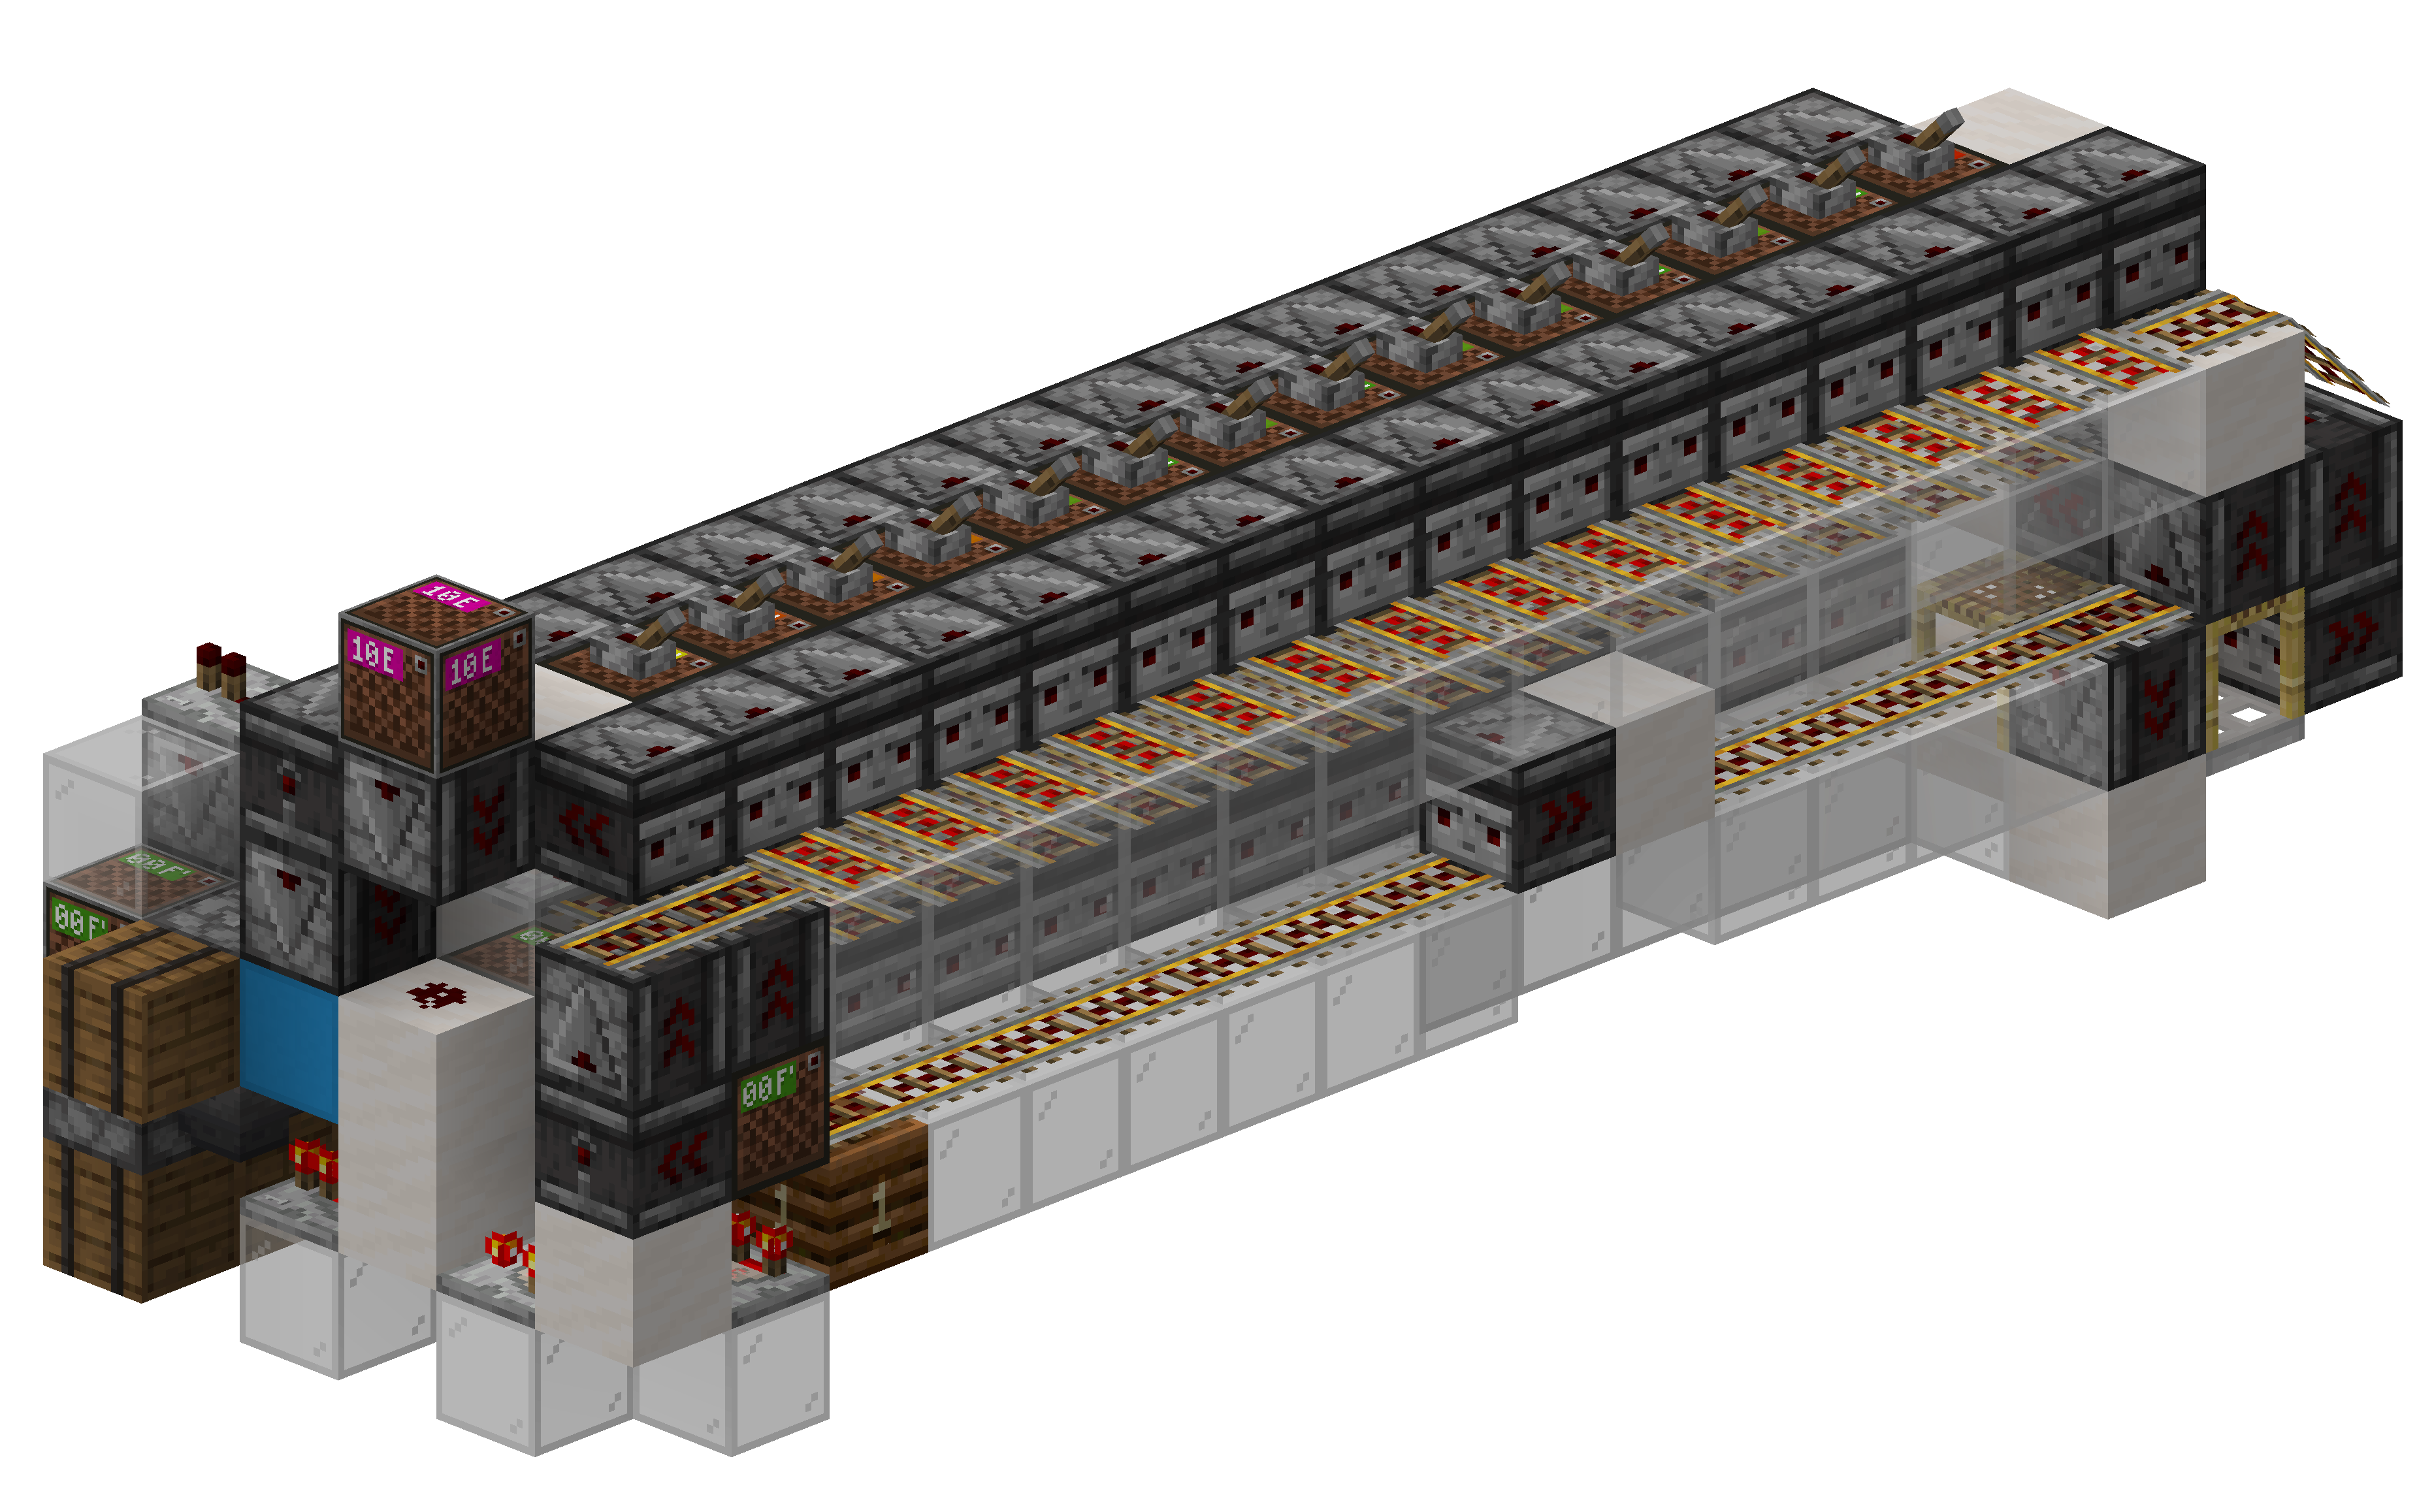
\includegraphics[width=0.48\textwidth]{area_render_56.png}
    \caption{\centering Merging Pair Optimizer}
\end{figure}

% For wide tables, a single column layout is better. It can be switched
% page-by-page.
\onecolumn

\section{Device Specifications}

\begin{table}[h]
    \caption{Inputs}
    \begin{tabularx}{\textwidth}{l | c | X}
        \thickhline
        \textbf{Name} & \textbf{Range} & \textbf{Description} \\
        \hline
        Box inputs 1-14 & Box & Input boxes categorized by fill level  \\
        \hline
        Start & Pulse & Starts outputting pairs of boxes at 16gt per pair  \\
        \thickhline
\end{tabularx}
\end{table}

\begin{table}[h]
    \caption{Outputs}
    \begin{tabularx}{\textwidth}{l | c | X}
        \thickhline
        \textbf{Name} & \textbf{Range} & \textbf{Description} \\
        \hline
        Paired box 1-2 & Box & Outputs paired boxes \\
        \hline
        Unpaired box & Box & Outputs unpaired box \\
        \thickhline
\end{tabularx}
\end{table}

\begin{table}[h]
    \caption{Device Specifications}
    \begin{tabularx}{\textwidth}{l | c c c | c | X}
        \thickhline
        \textbf{Parameter} & \textbf{Min.} & \textbf{Typ.} & \textbf{Max.} &
        \textbf{Unit} & \textbf{Conditions} \\
        \hline
        Throughput  & 16 & - & - & gt & Normal Usage \\
        \hline
        MC Version & 1.14 & 1.19.3 & - & MCV & Latest version at time of writing: 1.20.4\\
        \hline
        Dimensions & & 6 x 6 x 19 & & Blocks & \\
        \thickhline
\end{tabularx}
\end{table}
\newpage
\section{Testing Data}
\begin{table}[h]
\caption{Executed Tests}
\begin{tabularx}{\textwidth}{l | X}
    \thickhline
    \textbf{Test} & \textbf{Result} \\
    \hline
    Pairing test & Device was able to pair according to most-least pairing algorithm with random box input. \\
    \thickhline
\end{tabularx}
\end{table}

\section{Download Information}
\begin{table}[h]
    \caption{Download Information}
    \begin{tabularx}{\textwidth}{l | l | l | X}
        \thickhline
        \textbf{Identifier} & \textbf{MC} & \textbf{File} & \textbf{Description} \\
        \hline
        MG01 & 1.19.3 & \href{https://github.com/Soontech-Annals/Archive/blob/8413f90a054b6c415703bae02badeba7541344f6/Archive/merging/MG01\%20Merging\%20Pair\%20Optimizer/MG01\_Merging\_Pair\_Optimizer.litematic?raw=1}{MG01\_Merging\_Pair\_Optimizer.litematic} & Schematic of device. \\
        \hline
        MG01 & 1.19.3 & \href{https://github.com/Soontech-Annals/Archive/blob/8413f90a054b6c415703bae02badeba7541344f6/Archive/merging/MG01\%20Merging\%20Pair\%20Optimizer/MG01S\_Merging\_Pair\_Optimizer\_With\_Sorter.litematic?raw=1}{MG01S\_Merging\_Pair\_Optimizer\_With\_Sorter.litematic} & Schematic of device with fill level sorter. \\
        \hline
        \thickhline
    \end{tabularx}
\end{table}

\newpage
\section{Related Components}
\begin{table}[h]
    \caption{Related Components}
    \begin{tabularx}{\textwidth}{ l | l }
        \thickhline
        \textbf{Identifier} & \textbf{Description} \\
        \hline
        LC05 & Pairer based on stateless find nearest device. \\
        \thickhline
    \end{tabularx}
\end{table}
\end{document}

